In order to make good decisions for imputation, it is important to understand how it impacts prediction. To gain a better understanding of this issue, we solve a very simple case of cross-validated regression with missing data. Although quite restrictive, this situation provides some insights into the way that missing data impacts prediction performance.

	\section{Problem set-up}
We place ourselves in a linerar regression setup with cross-validation (cf Chapter \ref{validation}). The data is split between a training dataset $X_A, y_A$ and validation dataset $X_V, y_V$. We use the multi-agent framework described in \ref{framework}.
		\subsection{Notations}
			\subsubsection{God's data}
The response variable is a noisy linear combination of the covariates in $X$:
\begin{equation*}
\tilde{X}_A = 
\begin{pmatrix}
x_{11} & x_{12} \\
\vdots & \vdots \\
x_{n1} & x_{n2}
\end{pmatrix}
\quad \mathrm{and} \quad
y_A = X_A \beta + \epsilon_A
\quad \mathrm{with} \quad
\epsilon_A \sim \mathcal{N}(0, \sigma^2)
\end{equation*}
\begin{equation*}
\tilde{X_V} = 
\begin{pmatrix}
x_{11}^V & x_{12}^V \\
\vdots & \vdots \\
x_{n_V1} & x_{n_V2}
\end{pmatrix}
\quad \mathrm{and} \quad
y_V = X_V \beta + \epsilon_V
\quad \mathrm{with} \quad
\epsilon_V \sim \mathcal{N}(0, \sigma^2)
\end{equation*}

			\subsubsection{Observed data}
The observed data is God's data with some missing values. Specifically, some observations are missing from the first column of each dataset.  We observe the full $y^A$, but the covariate matrices we actually have access to are:
\begin{equation*}
X_A = 
\begin{pmatrix}
? & x_{12} \\
\vdots & \vdots \\
? & x_{k_A2} \\
x_{(k_A+1)1} & x_{(k_A+1)2}\\
\vdots & \vdots \\
x_{n1} & x_{n2}
\end{pmatrix}
\end{equation*}

which is sent to the Imputer, and

\begin{equation*}
X_V = 
\begin{pmatrix}
? & x_{12} \\
\vdots & \vdots \\
? & x_{k_V 2} \\
x_{(k_V+1)1} & x_{(k_V+1)2}\\
\vdots & \vdots \\
x_{n_V 1} & x_{n_V 2}
\end{pmatrix}
\end{equation*}

which is sent to the Practitioner. That is, there are $k_A$ and $k_v$ missing values in the datasets.

		\subsection{Imputed data and regression}
			\subsubsection{Principle}
The imputer fills in $X_A$ with imputed values, and instructs the Practitioner as to how to fill in $X_V$. The resulting filled in datasets are:

\begin{equation*}
\hat{X}_A = 
\begin{pmatrix}
\phi_1 & x_{12} \\
\vdots & \vdots \\
\phi_{k_A} & x_{k_A 2} \\
x_{(k_A+1)1} & x_{(k_A+1)2}\\
\vdots & \vdots \\
x_{n 1} & x_{n 2}
\end{pmatrix}
\quad \mathrm{and} \quad
\hat{X}_V = 
\begin{pmatrix}
\psi_1 & x_{12} \\
\vdots & \vdots \\
\psi_{k_V} & x_{k_V 2} \\
x_{(k_V+1)1} & x_{(k_V+1)2}\\
\vdots & \vdots \\
x_{n_V 1} & x_{n_V 2}
\end{pmatrix}
\end{equation*}

The $\phi$ values should depend only on the observed $X_A$, and the $\psi$ values on both $X_V$ and the imputer's indications. Then, $\hat{X}_A$ is sent by the imputer to the Analyst. The Analyst only has access to $\hat{X}_A$ and $y_A$. 
The end goal is to learn an estimator on the training set that minimizes the expected loss on the validation set:
$$
L(y_V, \hat{y}_V) = (y_V - \hat{y_V})^2
$$

In line with the principles of ERM and CV (cf \ref{validation}), the Analyst minimizes the equivalent quantity in the training set. Assuming a linear relationship between the covariantes and response, the least-squares estimate for $\beta$ is standard \cite{linear_regression}
$$
\hat{\beta}_n = (\hat{X}_A^T \hat{X}_A)^{-1} \hat{X}_A^T y_A 
$$

$\hat{\beta}$ is then transferred to the Practitioner who can use it to compute a prediction
$$\hat{y}_V (= \hat{X}_V \hat{\beta}_n $$

which will be compared to $y_V$:

$$L(\hat{y}_V, y_V) = \sum\limits_{i=1}^{n_V} (y_V^{(i)} - \hat{y}_V^{(i)})^2$$
Our end goal is to optimize this metric. 

In what we described above, the actions of the Analyst and the Practitioner are completely determined. On the other hand, we have not specified how the Imputer proceeds to the imputation. We want to investigate the effect of the choice of imputation on the expected loss:

$$R(\phi, \psi) = \mathbb{E}_{X_V^{miss}, X_A^{miss}, \epsilon_A, \epsilon_V}[(y_V^{(i)} - \hat{y}_V^{(i)})^2 \vert X_A, X_V, \phi, \psi]$$\footnote{Even though what we ultimately want is a decision rule for $\phi$ and $\psi$, they are only a function of the observed data $X_A$, $X_V$, which is fixed here. For simplicity of notation, we write $\phi$ and $\psi$ as constant values}


			\subsubsection{Distribution hypotheses}
Lastly, for this last expression to have any meaning, fix the distribution of $\tilde{X}$ the true data.

We assume $X \sim \pi$ where the lines of $X$ are independent and identically distributed, and that $\pi$ is known to the Imputer. This is unlikely in a real setting, but we explore the best-case scenario where we have all the necessary information to perform the imputation in order to isolate the error terms that are specific to the presence of missing data ---as opposed to bad imputation.

	\section{Partial resolution}
		\subsection{General loss}
To be able to estimate the expected loss, we break it up into several components. We first denote 
$$
\tilde{\beta}_n = (\tilde{X}_A^T \tilde{X}_A)^{-1} \tilde{X}_A^T y_A 
$$

the estimated parameter we would obtain if the training data were complete. We consider the loss for one given line of validation data $x_V = (x_V^1, x_V^2)$

\begin{align*}
L(y_V, \hat{y}_V) &= (y_V - \hat{y_V})^2 &\\
				   &= (\tilde{x}_V \beta + \epsilon_V - \hat{x}_V \hat{\beta}_n)^2 &\\
				   &= (\tilde{x}_V(\beta - \tilde{\beta}_n) + \tilde{x}_V (\tilde{\beta}_n - \hat{\beta}_n) + (\tilde{x}_V - \hat{x}_V) \hat{\beta}_n + \epsilon_V)^2 & \\
				   &= (\tilde{x}_V (\beta - \tilde{\beta}_n))^2 & (1) \\
				   & \quad + (\tilde{x}_V (\tilde{\beta}_n-\hat{\beta}_n))^2 &(2) \\
				   & \quad + ((\tilde{x}_V - \hat{x}_V) \hat{\beta}_n)^2 &(3) \\
				   & \quad + \tilde{x}_V (\beta - \tilde{\beta}_n) \tilde{x}_V (\tilde{\beta}_n - \hat{\beta}_n) & (4) \\
				   & \quad + \tilde{x}_V (\beta - \tilde{\beta}_n) (\tilde{x}_V - \hat{x}_V )\hat{\beta}_n & (5) \\
				   & \quad + \tilde{X}_V (\tilde{\beta}_n - \hat{\beta}_n) (\tilde{x}_V - \hat{x}_V) \hat{\beta}_n & (6)\\
				   & + \epsilon_V^2 &\\
				   & + \epsilon_V K
\end{align*}
Where $C$ is some term that will not matter (since it has zero expectation ---$\epsilon_V$ has zero expectation and is independent from the other terms). The risk we want to minimize is the expectation of this loss.
		\subsection{When the training set is fully observed}
			\subsubsection{Imputation}
The first thing we can do is to study the situation where the only missing data is in the validation set. In that case, $\tilde{X}_A = \hat{X}_A$ and so $\tilde{\beta}_n = \hat{\beta}_n$, and all we have to choose is $\psi$. In the previously computed loss, it means that terms $(2)$, $(4)$ and $(6)$ are zero.

Furthermore, 
\begin{align*}
\beta -\tilde{beta}_n &= \beta - (\tilde{X}_A^T \tilde{X}_A)-1 \tilde{X}_A^T (\tilde{X}_A \beta + \epsilon_A)\\
					&= (\tilde{X}_A^T \tilde{X}_A)-1 \tilde{X}_A^T \epsilon_A
\end{align*}
And 
\begin{align*}
(5) =  
\end{align*}

Furthermore, Cochran's theorem ensures that $(\beta - \tilde{\beta})$ and $\tilde{\beta}$ are independent so term $(5)$ can be factorized and will have zero expectation (since $(\beta - \tilde{\beta})$ has zero expectation).

Term $(1)$ depends only on the true values of $X_V$, independent of $psi$, so the choice of $\psi$  is not impacted by this term.

This leaves us with only term $(3)$, with expectation:
\begin{align*}
\mathbb{E}[((\tilde{X}_V-\hat{X}_V)\tilde{\beta})^2 \vert x^V_2, X_A] &= \mathbb{E}[(x_1^V - \psi)^2 \tilde{\beta}_1^2 \vert x^V_2, X_A] \\
													&= \mathbb{E}[\tilde{\beta}_1^2 \vert x^V_2, X_A] (\mathbb{E}[(x_1^V)^2\vert x^V_2, X_A] \\
													& \quad - 2\psi \mathbb{E}[x_1^V\vert x^V_2, X_A] + \psi^2)
\end{align*}
Once we are there, we can differentiate this expression to easily derive the optimal expression for $\psi$: $\hat{\psi} = \mathbb{E}[x_1^V\vert x^V_2]$, the conditional expectation of the missing value.

Incidentally, this does not use any assumption on the distribution of $X$: this would be true for any joint distribution we choose for the covariates.

			\subsubsection{Expected loss}
First note:
\begin{align*}
\eta = \beta - \tilde{\beta} &= \beta - (\tilde{X}_A^T \tilde{X}_A)^{-1} \tilde{X}_A^T y_A \\
		&= (\tilde{X}_A^T \tilde{X}_A)^{-1} \tilde{X}_A^T (\tilde{X}_A \beta + \epsilon_A) \\
		&= (\tilde{X}_A^T \tilde{X}_A)^{-1} \tilde{X}_A^T \epsilon_A
\end{align*}

That is, the difference between the estimated and real parameter is distributed following some centred normal distribution. Let us denote its covariance matrix by $S = \sigma^2 (\tilde{X}_A^T \tilde{X}_A)^{-1} $.

Now, term $(1)$ can be expressed as :
\begin{align*}
\mathbb{E}[(\tilde{X}_V \eta)^2 \vert x^V_2] &= \mathbb{E}[(x^V_1 \eta_1 + x^V_2 \eta_2)^2\vert x^V_2] \\
											&= S_{11} \mathbb{E}[(x^V_1)^2 \vert x^V_2]  + 2x^V_2 S_{12} \mathbb{E}[x^V_1 \vert x^V_2] + S_{22} (x^V_2)^2
\end{align*}

Term $(3)$ can be expressed as:
\begin{align*}
\mathbb{E}[((\tilde{X}_V - \hat{X}_V) \hat{\beta})^2 \vert x^V_2]&= \mathbb{E}[((x^V_1 - \hat{\psi})\tilde{\beta}_1)^2 \vert x^V_2] \\
									 &= \mathbb{E}[((x^V_1 - \hat{\psi})(\beta_1 + \eta_1))^2 \vert x^V_2] \\
									&= \beta_1^2 \text{Var}[x^V_1 \vert x^V_2] + S_{11}^2 \text{Var}[x^V_1 \vert x^V_2] 
\end{align*}

The terms from $(1)$ would be more or less the same if the test data were fully observed. They represent the impact on the prediction of the error made when estimating $\beta$.

 On the other hand, those from $(3)$ are both positive and unique to the incomplete case. They do not depend on the test data at all. The first term reflects how an error in the imputation of $X_V$ is amplified by the regression coefficient when predicting $y$. The second one shows how errors in the estimation of $\beta$ and of $X_V$ combine when predicting $y$.
 
 Most importantly, the least squares estimator is a strongly consistent one\cite{consistency_linreg}, which implies that the only error terms that matter with large $n$ are those that remain when $\eta$ is set to zero:
 $$ \beta_1^2 \text{Var}[x^V_1 \vert x^V_2] + \sigma^2 $$
 
 The missing data in the validation set adds a term that does not vanish for large $n$.
 
 \paragraph*{When there are more than two covariates}
 An important point is that in a context with more than two covariates, the conditional variance of an observation increases when the number of unobserved variables increases: this means that when the dimension increases, not only do new error terms appear, but the existing ones also increase.
 
 For $X_V$ with $p>2$ covariates, we denote $X_V^{\text{miss}}$ and $X_V^{\text{obs}}$ the missing and observed values in $X_V$. We can now write $(3)$ again:
 \begin{align*}
 \mathbb{E}[((\tilde{X}_V - \hat{X}_V)\beta)^2 \vert X_V^{\text{obs}}] &= 
 		\mathbb{E}[ (\sum \limits_{\substack{i=1 \\i \in X_V^{\text{miss}}}}^{p} (x_i^V - \hat{x}_i^V)\beta_i)^2 \vert X_V^{\text{obs}}] \\
 		&= \mathbb{E}[\sum \limits_{\substack{i=1 \\i \in X_V^{\text{miss}}}}^{p} \sum \limits_{\substack{j=1 \\j \in X_V^{\text{miss}}}}^{p}
 			(x^V_i - \hat{x}^V_i)(x^V_j - \hat{x}^V_j)\beta_i \beta_j \vert X_V^{\text{obs}}]
 \end{align*}
 
 If, as previously, we choose $\hat{x}^V_i = \mathbb{E}[x^V_i \vert X_V^{\text{obs}}]$, we end up with:
 \begin{align*}
 \mathbb{E}[((\tilde{X}_V - \hat{X}_V)\beta)^2 \vert X_V^{\text{obs}}] &= 
 	\sum \limits_{\substack{i,j=1 \\i,j \in X_V^{\text{miss}}}}^{p} \beta_i \beta_j Cov(x^V_i, x^V_j \vert X_V^{\text{obs}})
 \end{align*}

		\subsection{When the data is large and the training data is fully observed}
We can suppose that $n$ is large and that we know $\tilde{X_V}$. In that case, we can take the approximation that $\beta = \tilde{\beta}$, that is, the only error in the estimation of $\beta$ comes from the missing data in the training set. Then, the only error term that is nonzero is $(2)$:
$$ (\tilde{X}_V (\hat{\beta} - \tilde{\beta}))^2$$
\todo{To complete}
	\section{Analysis}
		\subsection{Implications}
\paragraph{Theoretical consequences}
If the results above are any indication as to how things go in more complex settings, there are some interesting implications. 

First, this confirms our intuition that using the conditional mean is the right thing to do to impute the validation data. This is important, especially as most imputation packages were made for multiple imputation and draw from the conditional distribution instead.

Second, there is a major asymmetry between the training and validation dataset: in the training set, every line works together with the others to help estimate some parameter. In particular, this means that even if all of the imputations are imperfect, with enough observations we can obtain a satisfactory estimate of the parameters (this is similar to the case of statistical inference with missing data, where under some assumptions the estimators are asymptotically consistent \cite{rubin_ignorability}). More data adds information, and even if it is incomplete it helps with the estimation.

The validation data is in a completely different situation. Missing data in the validation dataset adds error terms to the data that can be very large and do not vanish asymptotically. Intuitively, even if we have exactly the right $\beta$ for regression, any error in the estimation of the data will be directly reflected as a prediction error proportional to the regression coefficient, while in the training set this effect is much more indirect. Such errors are inevitable, even if we know the exact distribution of the data, because it is random. The expected loss will be the same for every line on the validation set (with the same missingness pattern), so adding more validation lines will do nothing to reduce the mean error if they also have missing data. This is important not only from the standpoint of model selection, but also because the validation error gives us an idea of how our model will perform on real-world data: missing data in the data we use for prediction can be a much more severe issue than missing data in our training database.

\paragraph{Implications for our data}

This could actually be a positive find. Take the example of Traumabase and haemorrhagic shock prediction: part of what our results mean is that the Traumabase can indeed be used to build a prediction tool, even if it has a significant amount of missing data. If the missing data is mostly due to errors of recording, this may mean that it is available in the real world when a doctor uses the tool: if the data used to make important predictions (that is, not a posteriori from the base but in a hospital when a patient needs care) can be kept full, then our estimates will have a chance of being very good, as long as we built our model with a large enough database.

The flip size, of course, is that when data is indeed missing from the validation dataset, there is little we can do to offset the resulting penalty. The missing value has a natural variability, even when controlling for every other observed variable, so even our best guess could have a high error. 

\subsection{Partial multiple imputation}
This suggests an idea that could help mitigate this drawback while keeping the computational cost rather low. Using $X_A$ the training data, we can estimate parameters $\phi, \psi, \beta$ as usual. Then, keeping these parameters constant, we can make draws from the conditional distribution of $X_V$ and make predictions on the datasets generated this way. Using the quantiles of these predictions, we can build intervals that approximate the possible location of the true value of $y$ and account for uncertainty. The idea behind this is that it is not necessary to multiply impute $X_A$ because with lare $n$ the estimated parameters will not really vary. It is also computationally intensive because it means we have to fit a new model for every imputed dataset. With our method, just one fit is needed and we only perform multiple predictions, which are usually cheaper.

To illustrate these results, we perform an analysis on some very simple simulated data, and check if the properties we derived are visible.
		\subsection{Verification on real and simulated data}
We ran an analysis on two sets of data:
\begin{enumerate}
\item A simulated dataset designed to respect the assumptions of our model: the $X$ data is generated as a multivariate normal for some random covariance matrix (with $p=10$ variables), and the response are obtained linearly by scalar product with some parameter $\beta$ (plus some noise)
\item A very simple real world dataset: the Abalone dataset. It is a regression dataset where the goal is to predict the age of a shell based on 7 measurements. It has no missing data and the covariates have high correlation.There are more that 4000 observations.
\end{enumerate}

On both dataset, we ran the following procedure:
\begin{itemize}
\item Split the data in a training and a validation datasets.
\item Perform one linear regression on the complete dataset.
\item Add some (30\%) missing data completely at random.
\item Impute the data by the mean, perform a regression.
\item Using the complete training data and the validation data with missing values, impute the data as a multivariate normal and perform a regression.
\item Using the training data data with missing values and the complete validation, impute the data as a multivariate normal and perform a regression.
\item Using both datasets with missing values, impute the data as a multivariate normal and perform a regression.
\item Compute the mean squared prediction error for each of the five regressions on the validation data.
\end{itemize}
		
This is repeated multiple times to smooth out the variability of the results. We do this for a broad range of $n$ values (for Abalone we select $n$ rows at random for the analysis, for the simulated data we generate $n$ rows each time).

The results are shown in Figure \ref{fig.linreg}. 

\begin{figure}[h]
  \centering
  \subbottom[Results for simulated data (log scale)]{%
    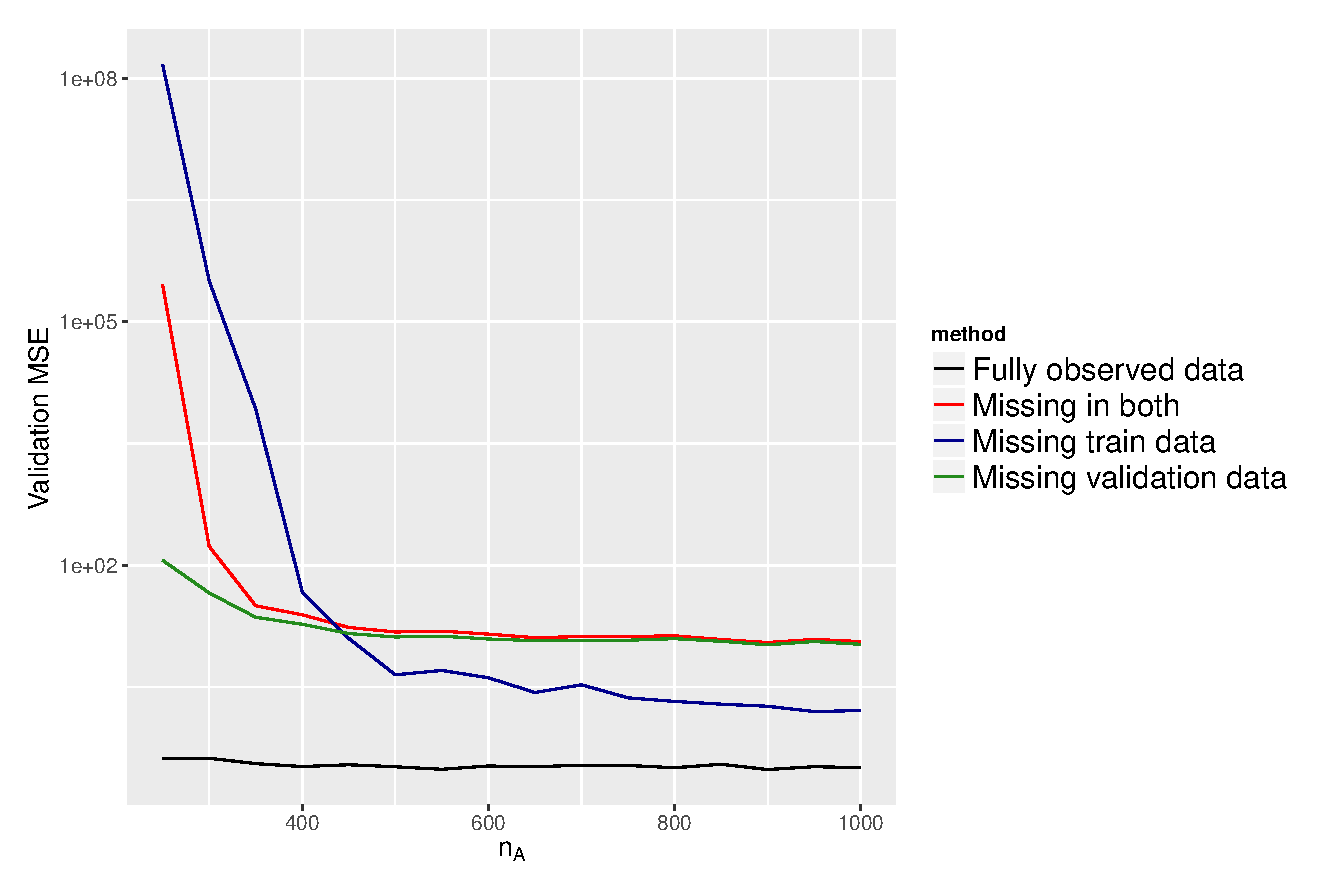
\includegraphics[scale=0.4]{Resources/linreg_sim}}\\
  \subbottom[Results for abalone data]{%
    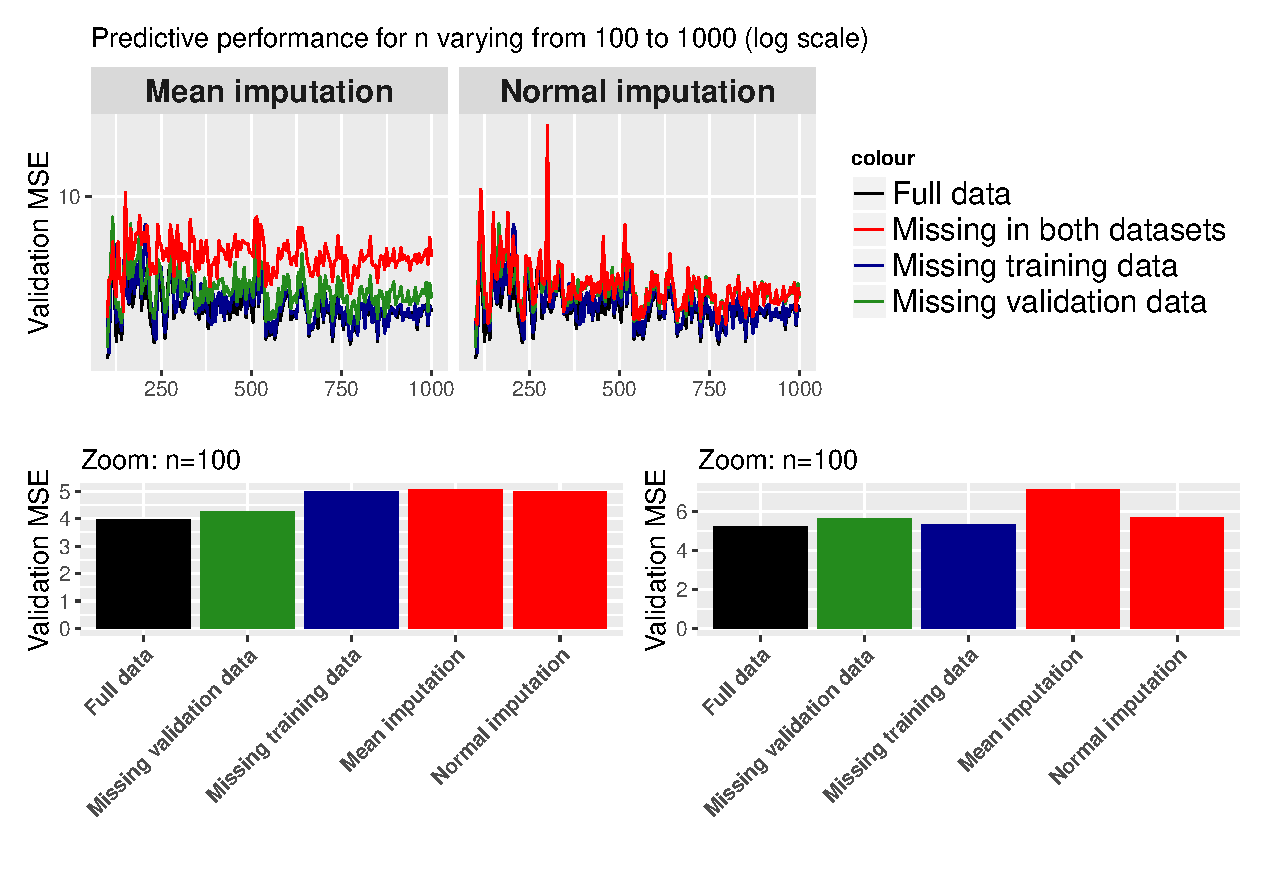
\includegraphics[scale=0.4]{Resources/linreg_abalone}}
  \caption{Impact of missing data in the train and validation set}
  \label{fig.linreg}  
\end{figure}

The trends are less visible in the Abalone data, most likely because the base error from model misspecification is higher so the relative variations are smaller. However, we can see some general trends emerge.

\textbf{For large $n$}, the results match our expectations. The error is much lower when the validation data is known, while there is almost no difference with and without knowing the real training data: with enough information we make up for the missing data when estimating the parameters. Even on the Abalone data (which is not really normally distributed), the normal imputation performs much better than imputation by the mean.

\textbf{For small $n$}, everything is very different. The first striking result is that the main error term comes from the missing data in the training set, this time. This makes sense, as for such a small $n$ it is very difficult to accurately estimate the covariance of the data, so missing values in the training data can seriously impact parameter estimation for the imputation. For the same reason, it is understandable that imputation by the mean works better than normal imputation in this context: with less parameters to estimate, we can at least have a fairly good estimation of the mean rather than a very bad estimation of both the mean and covariance. 

Throughout the spectrum of $n$, we also see that the imputation with missing data everywhere tends to match whichever is worse between the full training data and the full validation data. These values act as lower bounds for the quality of prediction.